\documentclass[12pt, letterpaper]{article}
\usepackage{graphicx}
\usepackage{hyperref}
\usepackage{xcolor}

\title{SENG 474 A02: Assignment 1 \\[1ex]
\large Binary Classification Experiments:
\large \textit{Decision Trees, Random Forests, and Neural Networks}}
\author{Sean McAuliffe, V00913346 }
\date{February 4th, 2023}
\graphicspath{{../../figures/}}

\begin{document}

\maketitle

\pagebreak
\tableofcontents
\pagebreak

\part*{Introduction}

\section{Background}

\paragraph*{}This report summarizes the results of a series of experiments
conducted to measure and compare the performance of three different methods of
binary classification: decision trees, random forests, and neural networks. For
each of these approaches a number of models were trained on a
\href{https://archive.ics.uci.edu/ml/datasets/adult}{\textcolor{blue}{\underline{provided dataset}}}
containing census information of american adults, with the goal of predicting
whether or not an individual makes more than \$50,000 a year.

\paragraph*{}Each experiment consisted of splitting the dataset into a
training set and a test set, and varying a single training hyperparameter of
interest while measuring the resulting performance of the model. Each experiment
produced a graph of the model training and test accuracy (or error) as a
function of the hyperparameter.

\paragraph*{}Some of the experiments tested  different combinations of
parameters such as optimizationm algorithms, and so did not produce a chart of
accuracy as a function of the hyperparameter because the possible parameter
values were categorical, not numerical. In these cases the results are
presented in a table.

\section{Environment \& Implementations}

\paragraph*{}The three classifier methods were not implemented from scratch for
the purposes of this assignment. Instead, the \textbf{scikit-learn} library was
used. The experiments were conudcted in Jupyter Notebooks running on a Python
3.10.6 kernel (not the default ipython kernel). The notebooks have been provided
with this report. An associated README file constains intructions for running
the notebooks in order to replicate the results.

\part*{Decision Trees}

\section{DT Hyperparameters}

\paragraph*{}Decision trees are a supervised learning method which can be used
for classification and regression. A tree consists of a number of nodes which
represent a question about some feature of the data, here the remaining examples
are split into children nodes according to some threshold of the feature value.
At leaf nodes, the model learns to predict a classification label by inspecting
the labels of the provided training examples which have ended up at this node
and using a majority vote. Future testing examples which have feature values
which lead to this leaf node will take on this predicted classification.

\paragraph*{}\textbf{Scikit-learn} provides a \textbf{DecisionTreeClassifier}
class which can be used to perform the binary classification experiment. The
following hyperparameters are of interest.

\begin{itemize}
    \item \textbf{criterion}: The function used to measure the quality of a
    split.
    \item \textbf{max\_depth}: The maximum depth of the tree.
    \item \textbf{ccp\_alpha}: Complexity parameter used for Minimal Cost Complexity
    pruning.
\end{itemize}

\section{Decision Tree Classifier Experiments}

\subsection{Maximum Tree Depth}

\paragraph*{Experiment 1:} The data was split according to a 80\% - 20\%
training-testing split. The maximum depth of the DTC was varied from 2-100.
For each value of max\_depth a new model was trained on the training data and 
scored against the testing data. The results are shown in Figure \ref{fig:dt1}.

\begin{figure}[ht]
    \centering
    \begin{minipage}{0.5\textwidth}
        \centering
        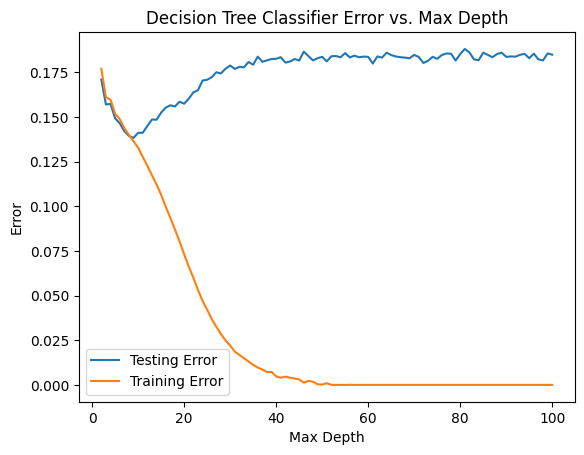
\includegraphics[width=\textwidth]{dt/dt2.png} % first figure itself
    \end{minipage}\hfill
    \begin{minipage}{0.5\textwidth}
        \centering
        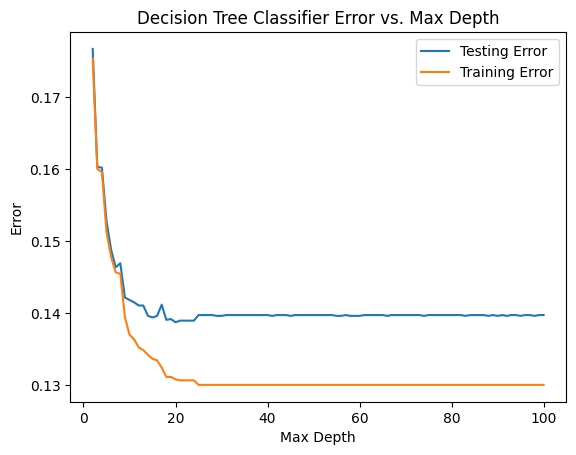
\includegraphics[width=\textwidth]{dt/dt4.png} % second figure itself
    \end{minipage}
    \caption{DTC Error Rate vs. Maximum Tree Depth (Top: w/o pruning,
            Bottom: w/ pruning)}
    \label{fig:dt1}
\end{figure}

\paragraph*{}The results of experiment 1 (without pruning) show a clear pattern
of overfitting. The training error decreases to near zero as the tree depth
increases. While the testing error initially decreases, but then quickly 
begins to rise and plateaus at a value of approximately 0.175. This is
seemingly prevented with the inclusion of post-pruning.

\paragraph*{}Minimal cost complexity post pruning is used here to prevent over-
fitting. This method of post pruning is included in the \textbf{DecisionTreeClassifier}
class in \textbf{scikit-learn} and is enabled by setting the \textbf{ccp\_alpha}
hyperparameter to a non-zero value (the default is zero). The optimal value of
\textbf{ccp\_alpha} was found in a later experiment and was then applied here.

\paragraph*{}The application of post pruning reduces the final testing error 
to approximately 0.14; a fairly significant improvement. The testing error plateaus
after a tree depth of approximately 20, and further increasing the depth does not
increase the testing error; suggesting that this method has successfully prevented
the model from overfitting.

\subsection{Complexity Parameter}

\paragraph*{Experiment 2:} The data was split according to a 80\% - 20\%
training-testing split. The complexity parameter \textbf{ccp\_alpha} of the DTC
was varied from 0-0.005. For each value of \textbf{ccp\_alpha} a new model was
trained on the training data and scored on the testing data. The results shown
in Figure \ref{fig:dt2}.

\begin{figure}[ht]
    \centering
    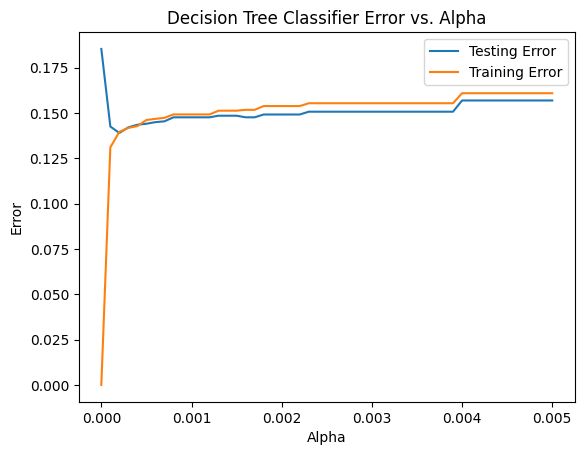
\includegraphics[width=\textwidth]{dt/dt6.png} % first figure itself
    \caption{DTC Error Rate vs. Complexity Parameter (Top: w/o pruning,
            Bottom: w/ pruning)}
    \label{fig:dt2}
\end{figure}

\paragraph*{}The results show that with no pruning (\textbf{ccp\_alpha} = 0.0)
the model overfits, with the training error near zero, and a relatively high
testing error. As the value of \textbf{ccp\_alpha} increases, the model
training and testing error converge on a value of approximately 0.15. The optimal
value is found to be approximately 0.0002. This value has been applied to the
other experiments in retrospect.

\paragraph*{}The depth of the tree resulting from trainig without prunning tends
to be around 54. The depth of the tree resulting from training with pruning
tends to be around 12. Reducing the total number of nodes in the tree from
10831 to 107. This is a significant improvement in the performance of the model.

\subsection{Proportion of Data in Training Set}
\paragraph*{Experiment 3:} The proportion of the data used for training was
varied from 10\% to 90\%. For each proportion a new DTC model was trained on 
the training set and scored on the testing set. In the results below the graph
plots the accuracy of the model, not its error. The results are shown in
Figure \ref{fig:dt3}.

\begin{figure}[ht]
    \centering
    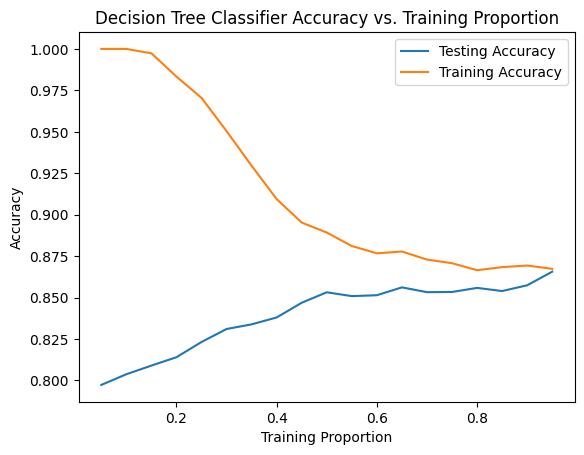
\includegraphics[width=\textwidth]{dt/dt7.png} % first figure itself
    \caption{DTC Accuracy vs. Proportion of Data in Training Set (w/ Pruning)}
    \label{fig:dt3}
\end{figure}

\paragraph*{}As an extension of this experiment, the model accuracy was again
measured with respect to the proportion of data in the training set, but this
time no post-pruning was used. The results (shown in figure \ref{fig:dt4})
appear to show that the DTC model overfits when allowed to go to an arbitrary
depth, and that the degree of overfitting is not influenced much by the training \/
testing set proportions. I had expected larger training sets to be harder to overfit-to,
but this does not appear in the results.

\begin{figure}
    \centering
    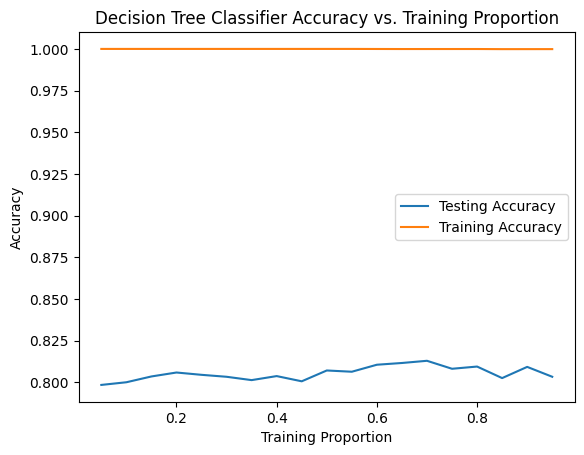
\includegraphics[width=\textwidth]{dt/dt8.png} % first figure itself
    \caption{DTC Accuracy vs. Proportion of Data in Training Set (No Pruning)}
    \label{fig:dt4}
\end{figure}

\subsection{Criterion}
\paragraph*{Experiment 4:} The criterion used for splitting was varied between
\textbf{gini}, \textbf{log loss}, and \textbf{entropy}. For each criterion a
new DTC model was trained on the training set and scored on the testing set. 
The results are shown below. The results appear to imply that entropy and log-loss
crieterion are more sensitive to overfitting, and that the best testing accuracy
can be achieved with the gini criterion.

\begin{verbatim}
Training Accuracy:
    Gini:       0.86944
    Entropy:    0.91187
    Log Loss:   0.91149

Testing Accuracy:
    Gini:       0.85682
    Entropy:    0.84002
    Log Loss:   0.83957
\end{verbatim}

\part*{Random Forests}

\section{RF Hyperparameters}

\paragraph*{}Random Forests are an ensemble classification method which consrtuct
many Decision Trees, each one trained on a bootstrap sample (a subset of the full
training set). Each tree is trained on a random subset of the features. The final
prediction of the Random Forest is made by averaging the predictions of each of 
its Decision Trees. This method can be very effective at certain kinds of problems.

\paragraph*{}\textbf{Scikit-learn} provides a \textbf{RandomForestClassifier} class
which is used in this section. The hyperparameters of the Random Forest Classifier
which are of interest in the following experiments are:

\begin{itemize}
    \item \textbf{n\_estimators}: The number of trees in the forest.
    \item \textbf{max\_depth}: The maximum depth of each tree.
    \item \textbf{max\_features}: The max. number of features to consider for a split.
    \item \textbf{max\_samples}: The max. number of samples drawn from the training set to train a single estimator.
    \item \textbf{min\_samples\_split}: The min. number of samples required to split an internal node.
\end{itemize}

\section{Random Forest Classifier Experiments}

\subsection{Forest Size}

\paragraph*{Experiment 5:} The number of trees in the forest was
varied from 2 to 200 in steps of 5. For each value of \textbf{n\_estimators} a new
Random Forest model was trained on the training set and scored on the testing set.
This experiment used an 80\% - 20\% training-testing split. The results are shown
in Figures \ref{fig:rf1}, \ref{fig:rf2}, and \ref{fig:rf3}.

\begin{figure}[ht]
    \centering
    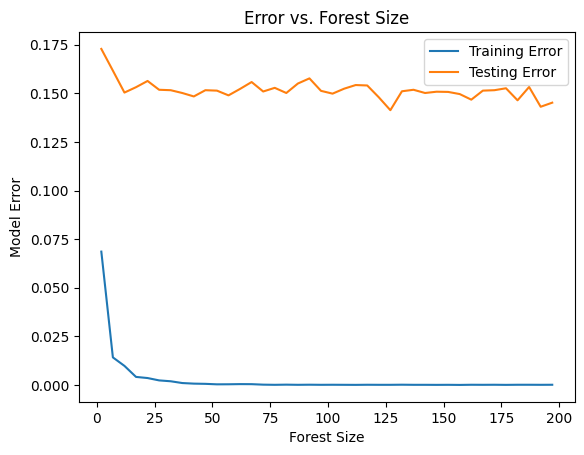
\includegraphics[width=\textwidth]{rf/rf2.png} % first figure itself
    \caption{RF Error vs. Forest Size (dynamic set)}
    \label{fig:rf1}
\end{figure}

\begin{figure}[ht]
    \centering
    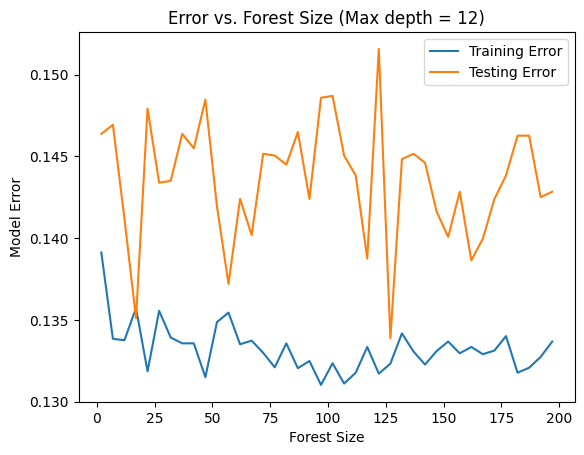
\includegraphics[width=\textwidth]{rf/rf3.png} % first figure itself
    \caption{RF Error vs. Forest Size (max\_depth = 12, dynamic set)}
    \label{fig:rf2}
\end{figure}

\begin{figure}[ht]
    \centering
    \includegraphics[width=\textwidth]{rf/rfx.png} % first figure itself
    \caption{RF Error vs. Forest Size (max\_depth = 12, static set)}
    \label{fig:rf3}
\end{figure}

\paragraph*{}The results shown in Figures \ref{fig:rf1} and \ref{fig:rf2} show 
the accuracy of models each of which was trained and scored on a differntly shuffled
dataset (dynamic set) to maximize the randomness between iterations of \textbf{n\_estimators}.
The results shown in Figure \ref{fig:rf3} show the accuracy of models each of which
was trained on the same dataset (static set) to minimize the randomness between
iterations of \textbf{n\_estimators}

\paragraph*{}It seems that changing the shuffled order of the dataset introduces
a lot of variabiltiy in the accuracy of the resulting mode. This implies that some
sequences of training examples are 'lucky', producing more accurate models. 

\paragraph*{}The results of Figure \ref{fig:rf3} does not show an overfitting pattern
to the same degree as was observed in the DTC experiments without pruning. The
training and testing accuracy are different, but the difference does not appear to
be increasing as the size of the forest increases.

\paragraph*{} A curve of best fit was fit to the accuracy data from this experiment,
and it was found that the larger the size of the forest, the better the accuracy of
the model. However, there is clearly a point of diminshing returns after about
40-50 trees. This is shown in Figure \ref{fig:rf4}. Future experiments will used
50 estimators, since this is the point of diminshing returns.

\begin{figure}[ht]
    \centering
    \begin{verbatim}
        maximum: 199.9984637007033 0.8583552232362794
    \end{verbatim}
    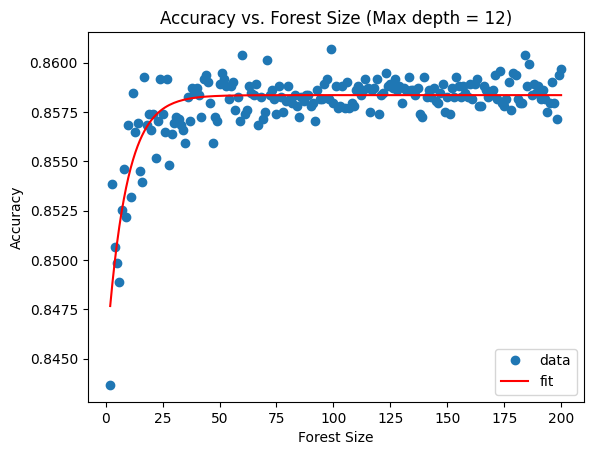
\includegraphics[width=\textwidth]{rf/rf6.png} % first figure itself
    \caption{RFC Accracy vs. Forest Size (max\_depth = 12, static set)}
    \label{fig:rf4}
\end{figure}
\pagebreak

\subsection{Maximum Number of Features, d'}
\paragraph*{Experiment 6:}The data was split into 80\% training and 20\% testing
sets. The maximum number of features a tree could consider for a split was varied
from 1 to 104 (the maximum number of features in the data). For each value of 
\textbf{max\_features} a new RFC model was trained on the training set and scored
on the testing set. The results are shown in Figure \ref{fig:rf5}.

% \begin{figure}[ht]
%     \centering
%     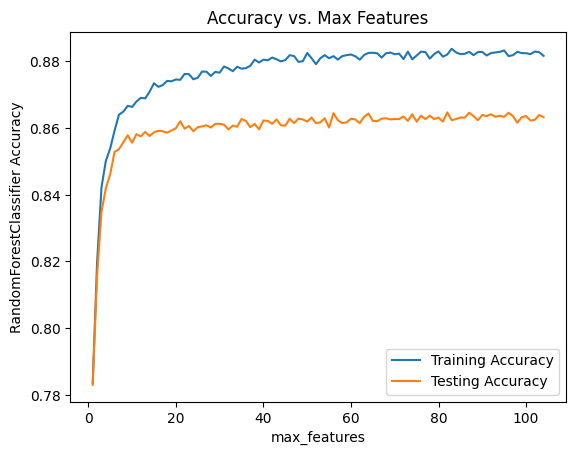
\includegraphics[width=\textwidth]{rf/rf8.png} % first figure itself
%     \caption{RF Error vs. Forest Size (max\_depth = 12, static set)}
%     \label{fig:rf5}
% \end{figure}

\begin{figure}[ht]
    \centering
    \begin{minipage}{0.5\textwidth}
        \centering
        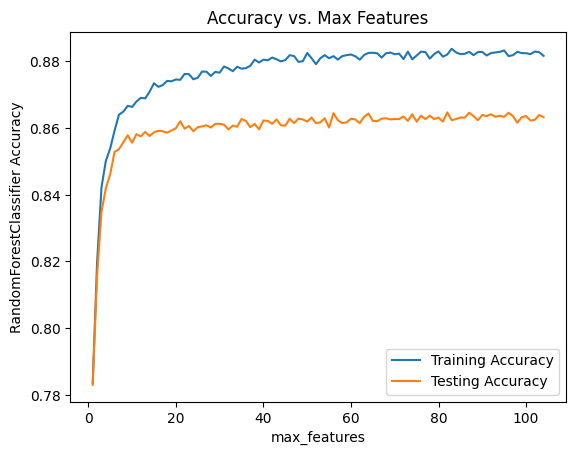
\includegraphics[width=\textwidth]{rf/rf8.png} % first figure itself
    \end{minipage}\hfill
    \begin{minipage}{0.5\textwidth}
        \centering
        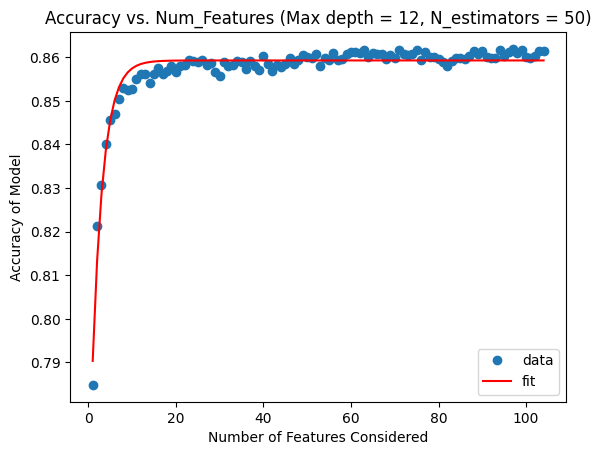
\includegraphics[width=\textwidth]{rf/rf9.png} % second figure itself
    \end{minipage}
    \caption{RFC Accuracy vs. Max. Features (max\_depth = 12)}
    \label{fig:rf5}
\end{figure}

\paragraph*{}It seems that the benefit of including more features increases without
bound. However, there is clearly a point of diminshing returns which begins after
approximately 20 features. In this experiment the maximum accuracy was achieved
with 90 features, so this value will be used in subsequent experiments. 90 features
is larger than the default of $\sqrt{104} \approx 10$.

\subsection{Bootstrap Sample Size}
\paragraph*{Experiment 7:}This experient varied the size of the randomly selected
bootstrap sample on which each tree is trained. The default size is the size of the
training set. The data was split into 80\% training and 20\% testing sets. The
\textbf{max\_samples} parameter was varied from 0.01 to 1, representing the fraction
of the training set which should be used to construct the bootstrap sample (where
examples are drawn from the broader training set with replacement). The
results are shown in Figure \ref{fig:rf6}.

\begin{figure}[ht]
    \centering
    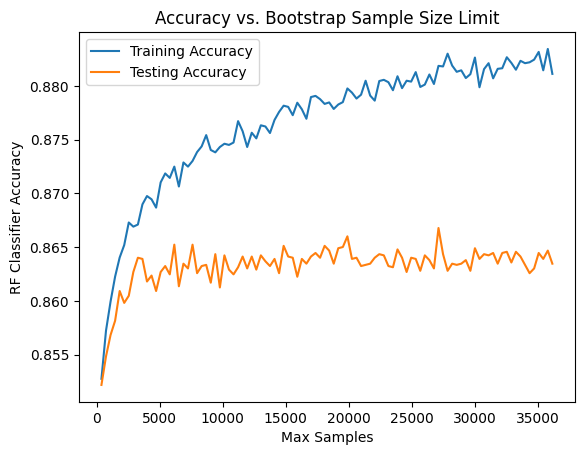
\includegraphics[width=\textwidth]{rf/rf10.png} % first figure itself
    \caption{RFC Accuracy vs Bootstrap Sample Size}
    \label{fig:rf6}
\end{figure}

\paragraph*{}The results of this experiment show that the accuracy of the model
increases as the size of the bootstrap sample increases. However, there is a point
of diminishing returns at approximately 3500 samples.

\subsection{Minimum Number of Samples to Split}

\paragraph*{Experiment 8:}This experiment varied the minimum number of samples
required to split an internal node. The data was split into 80\% training and
20\% testing sets. The \textbf{min\_samples\_split} parameter was varied from 1 to
10,000 in steps of 10. Having a very small value for this parameter allows the tree
to very finely tune to the training data, but may lead to overfitting to the particular
training examples it has seen. Increasing the value of this parameter prevents the
model from creating deeper trees which split on very small subsets of the data.
The results are shown in Figure \ref{fig:rf7}.

\begin{figure}[ht]
    \centering
    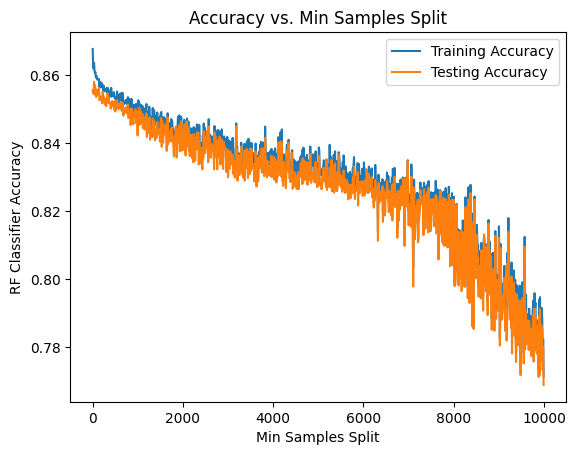
\includegraphics[width=\textwidth]{rf/rf12.png} % first figure itself
    \caption{RFC Accuracy vs Min. \# Samples to Split}
    \label{fig:rf7}
\end{figure}

\paragraph*{}The results show the overal random forest accurcy as a function
of the minimum number of samples required for a tree to split on an internal node.
The results show that there is no benefit in terms of model accuracy, to increasing
the value of this paramter. The best accuracy is achieved at the minimum value of 2.
For large models, there may be performance reasons for using a larger value for this
parameter.

\subsection{Out of Bag Error}
\paragraph*{Experiment 9:}In this experiment a method for measuring the OOB error
was implemented. The OOB error is the error of the model, using the majority vote
among only those trees in the forest which were not trained on a particular example.

\paragraph*{}The OOB implementation used the provided sample code to retrieve a list
of indices for each tree in the forest, specifying which examples were not used
to train that tree. The predictions of each tree were collected and averaged to produce
an overall prediction for the model.

\paragraph*{\textbf{OOB Implementation}}\textit{as shown in a1\_rf.ipynb}

\begin{verbatim}
def get_rf_prediction(rf, X):
    unsampled_i = find_unsampled_indices(...)
    estimators = rf.estimators_
    rf_predictions = []
    for i, x in enumerate(X):
        e_predictions = []
        for j, e in enumerate(estimators):
            if i in unsampled_i[j]:
                e_predictions.append(e.predict(x.reshape(1, -1)))
            else:
                pass
        avg_prediction = np.mean(e_predictions)
        if avg_prediction >= 0.5:
            rf_predictions.append(1)
        else:
            rf_predictions.append(0)
    return rf_predictions

def score_rf(predictions, y):
    correct = 0
    for p, y in zip(predictions, y):
        if p == y:
            correct += 1
    return correct / len(predictions)
\end{verbatim}

\paragraph*{}The OOB error was measured and plotted against the size of the random
forest. The results are shown below in Figure \ref{fig:rf8}. The OOB error does seem
to broadly follow the same trend as the test error, particularly for higher numbers
of estimators. However, the OOB error is always higher than the test error.


\begin{figure}[ht]
    \centering
    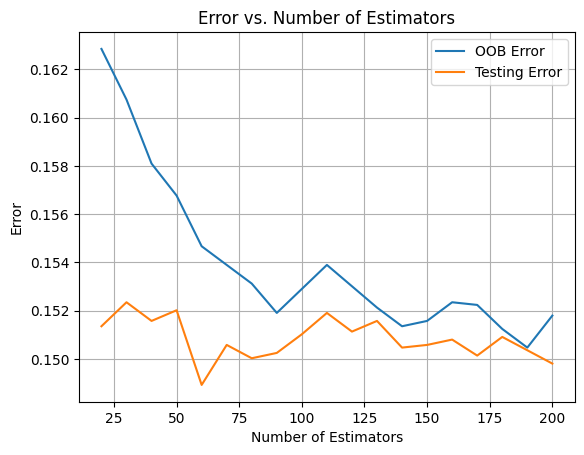
\includegraphics[width=\textwidth]{rf/rf14.png} % first figure itself
    \caption{RFC OOB Error vs. Number of Estimators}
    \label{fig:rf8}
\end{figure}


\pagebreak
\part*{Neural Networks}

\section{NN Hyperparameters}

\paragraph*{}Neural Networks (or Multi-Layer Perceptrons in scikit-learn vernacular)
are a powerful class of machine learning models which can be used for classification.
Neural Networks are highly generalizable and are able to learn complicated non-linar
relationships, and can approximate any function arbitraryily well (with enough hidden-layer nodes).

\paragraph*{}The experiments in this section will primarily use the suggestion network
architecture of 3 layers (1 input layer of 104 nodes, 1 hidden layer of a variable number 
of nodes, and one output layer, representing the predicted class label).

\paragraph*{}\textbf{Scikit-learn} provides a \textbf{MLPClassifier} class
which is used in this section. The hyperparameters of the MLP Classifier
which are of interest in the following experiments are:

\begin{itemize}
    \item \textbf{n\_estimators}: The number of trees in the forest.
    \item \textbf{max\_depth}: The maximum depth of each tree.
    \item \textbf{max\_features}: The max. number of features to consider for a split.
    \item \textbf{max\_samples}: The max. number of samples drawn from the training set to train a single estimator.
    \item \textbf{min\_samples\_split}: The min. number of samples required to split an internal node.
\end{itemize}

\section{Random Forest Classifier Experiments}

\subsection{Forest Size}

\paragraph*{Experiment 5:}

\paragraph*{}Test

\end{document}